\documentclass[11pt,a4paper,]{article}
\usepackage{lmodern}

\usepackage{amssymb,amsmath}
\usepackage{ifxetex,ifluatex}
\usepackage{fixltx2e} % provides \textsubscript
\ifnum 0\ifxetex 1\fi\ifluatex 1\fi=0 % if pdftex
  \usepackage[T1]{fontenc}
  \usepackage[utf8]{inputenc}
\else % if luatex or xelatex
  \usepackage{unicode-math}
  \defaultfontfeatures{Ligatures=TeX,Scale=MatchLowercase}
\fi
% use upquote if available, for straight quotes in verbatim environments
\IfFileExists{upquote.sty}{\usepackage{upquote}}{}
% use microtype if available
\IfFileExists{microtype.sty}{%
\usepackage[]{microtype}
\UseMicrotypeSet[protrusion]{basicmath} % disable protrusion for tt fonts
}{}
\PassOptionsToPackage{hyphens}{url} % url is loaded by hyperref
\usepackage[unicode=true]{hyperref}
\hypersetup{
            pdftitle={Corona Virus Report},
            pdfborder={0 0 0},
            breaklinks=true}
\urlstyle{same}  % don't use monospace font for urls
\usepackage{geometry}
\geometry{a4paper, centering, text={16cm,24cm}}
\usepackage[style=authoryear-comp,]{biblatex}
\addbibresource{references.bib}
\usepackage{longtable,booktabs}
% Fix footnotes in tables (requires footnote package)
\IfFileExists{footnote.sty}{\usepackage{footnote}\makesavenoteenv{long table}}{}
\usepackage{graphicx,grffile}
\makeatletter
\def\maxwidth{\ifdim\Gin@nat@width>\linewidth\linewidth\else\Gin@nat@width\fi}
\def\maxheight{\ifdim\Gin@nat@height>\textheight\textheight\else\Gin@nat@height\fi}
\makeatother
% Scale images if necessary, so that they will not overflow the page
% margins by default, and it is still possible to overwrite the defaults
% using explicit options in \includegraphics[width, height, ...]{}
\setkeys{Gin}{width=\maxwidth,height=\maxheight,keepaspectratio}
\IfFileExists{parskip.sty}{%
\usepackage{parskip}
}{% else
\setlength{\parindent}{0pt}
\setlength{\parskip}{6pt plus 2pt minus 1pt}
}
\setlength{\emergencystretch}{3em}  % prevent overfull lines
\providecommand{\tightlist}{%
  \setlength{\itemsep}{0pt}\setlength{\parskip}{0pt}}
\setcounter{secnumdepth}{5}

% set default figure placement to htbp
\makeatletter
\def\fps@figure{htbp}
\makeatother


\title{Corona Virus Report}

%% MONASH STUFF

%% CAPTIONS
\RequirePackage{caption}
\DeclareCaptionStyle{italic}[justification=centering]
 {labelfont={bf},textfont={it},labelsep=colon}
\captionsetup[figure]{style=italic,format=hang,singlelinecheck=true}
\captionsetup[table]{style=italic,format=hang,singlelinecheck=true}


%% FONT
\RequirePackage{bera}
\RequirePackage[charter,expert,sfscaled]{mathdesign}
\RequirePackage{fontawesome}

%% HEADERS AND FOOTERS
\RequirePackage{fancyhdr}
\pagestyle{fancy}
\rfoot{\Large\sffamily\raisebox{-0.1cm}{\textbf{\thepage}}}
\makeatletter
\lhead{\textsf{\expandafter{\@title}}}
\makeatother
\rhead{}
\cfoot{}
\setlength{\headheight}{15pt}
\renewcommand{\headrulewidth}{0.4pt}
\renewcommand{\footrulewidth}{0.4pt}
\fancypagestyle{plain}{%
\fancyhf{} % clear all header and footer fields
\fancyfoot[C]{\sffamily\thepage} % except the center
\renewcommand{\headrulewidth}{0pt}
\renewcommand{\footrulewidth}{0pt}}

%% MATHS
\RequirePackage{bm,amsmath}
\allowdisplaybreaks

%% GRAPHICS
\RequirePackage{graphicx}
\setcounter{topnumber}{2}
\setcounter{bottomnumber}{2}
\setcounter{totalnumber}{4}
\renewcommand{\topfraction}{0.85}
\renewcommand{\bottomfraction}{0.85}
\renewcommand{\textfraction}{0.15}
\renewcommand{\floatpagefraction}{0.8}


%\RequirePackage[section]{placeins}

%% SECTION TITLES


%% SECTION TITLES (NEW: Changing sections and subsections color)
\RequirePackage[compact,sf,bf]{titlesec}
\titleformat*{\section}{\Large\sf\bfseries\color[rgb]{0.8, 0.7, 0.1 }}
\titleformat*{\subsection}{\large\sf\bfseries\color[rgb]{0.8, 0.7, 0.1 }}
\titleformat*{\subsubsection}{\sf\bfseries\color[rgb]{0.8, 0.7, 0.1 }}
\titlespacing{\section}{0pt}{2ex}{.5ex}
\titlespacing{\subsection}{0pt}{1.5ex}{0ex}
\titlespacing{\subsubsection}{0pt}{.5ex}{0ex}


%% TITLE PAGE
\def\Date{\number\day}
\def\Month{\ifcase\month\or
 January\or February\or March\or April\or May\or June\or
 July\or August\or September\or October\or November\or December\fi}
\def\Year{\number\year}

%% LINE AND PAGE BREAKING
\sloppy
\clubpenalty = 10000
\widowpenalty = 10000
\brokenpenalty = 10000
\RequirePackage{microtype}

%% PARAGRAPH BREAKS
\setlength{\parskip}{1.4ex}
\setlength{\parindent}{0em}

%% HYPERLINKS
\RequirePackage{xcolor} % Needed for links
\definecolor{darkblue}{rgb}{0,0,.6}
\RequirePackage{url}

\makeatletter
\@ifpackageloaded{hyperref}{}{\RequirePackage{hyperref}}
\makeatother
\hypersetup{
     citecolor=0 0 0,
     breaklinks=true,
     bookmarksopen=true,
     bookmarksnumbered=true,
     linkcolor=darkblue,
     urlcolor=blue,
     citecolor=darkblue,
     colorlinks=true}

\usepackage[showonlyrefs]{mathtools}
\usepackage[no-weekday]{eukdate}

%% BIBLIOGRAPHY

\makeatletter
\@ifpackageloaded{biblatex}{}{\usepackage[style=authoryear-comp, backend=biber, natbib=true]{biblatex}}
\makeatother
\ExecuteBibliographyOptions{bibencoding=utf8,minnames=1,maxnames=3, maxbibnames=99,dashed=false,terseinits=true,giveninits=true,uniquename=false,uniquelist=false,doi=false, isbn=false,url=true,sortcites=false}

\DeclareFieldFormat{url}{\texttt{\url{#1}}}
\DeclareFieldFormat[article]{pages}{#1}
\DeclareFieldFormat[inproceedings]{pages}{\lowercase{pp.}#1}
\DeclareFieldFormat[incollection]{pages}{\lowercase{pp.}#1}
\DeclareFieldFormat[article]{volume}{\mkbibbold{#1}}
\DeclareFieldFormat[article]{number}{\mkbibparens{#1}}
\DeclareFieldFormat[article]{title}{\MakeCapital{#1}}
\DeclareFieldFormat[article]{url}{}
%\DeclareFieldFormat[book]{url}{}
%\DeclareFieldFormat[inbook]{url}{}
%\DeclareFieldFormat[incollection]{url}{}
%\DeclareFieldFormat[inproceedings]{url}{}
\DeclareFieldFormat[inproceedings]{title}{#1}
\DeclareFieldFormat{shorthandwidth}{#1}
%\DeclareFieldFormat{extrayear}{}
% No dot before number of articles
\usepackage{xpatch}
\xpatchbibmacro{volume+number+eid}{\setunit*{\adddot}}{}{}{}
% Remove In: for an article.
\renewbibmacro{in:}{%
  \ifentrytype{article}{}{%
  \printtext{\bibstring{in}\intitlepunct}}}

\AtEveryBibitem{\clearfield{month}}
\AtEveryCitekey{\clearfield{month}}

\makeatletter
\DeclareDelimFormat[cbx@textcite]{nameyeardelim}{\addspace}
\makeatother

\author{\sf\Large\textbf{ Jimmy Effendy}\\ {\sf\large B.Com\\[0.5cm]} \sf\Large\textbf{ Brendi Ang}\\ {\sf\large BSc\\[0.5cm]} \sf\Large\textbf{ Reports XXXX}\\ {\sf\large XXX\\[0.5cm]} \sf\Large\textbf{ XXX XXX}\\ {\sf\large XXX\\[0.5cm]}}

\date{\sf\Date~\Month~\Year}
\makeatletter
\lfoot{\sf Effendy, Ang, XXXX, XXX: \@date}
\makeatother


%%%% PAGE STYLE FOR FRONT PAGE OF REPORTS

\makeatletter
\def\organization#1{\gdef\@organization{#1}}
\def\telephone#1{\gdef\@telephone{#1}}
\def\email#1{\gdef\@email{#1}}
\makeatother
  \organization{Australian Government COVID19}

  \def\name{Our consultancy \newline add names \&\newline add names}

  \telephone{(03) 9905 2478}

  \email{questions@company.com}                 %NEW: New email addresss

\def\webaddress{\url{http://company.com/stats/consulting/}} %NEW: URl
\def\abn{12 377 614 630}                                    % NEW: ABN
\def\logo{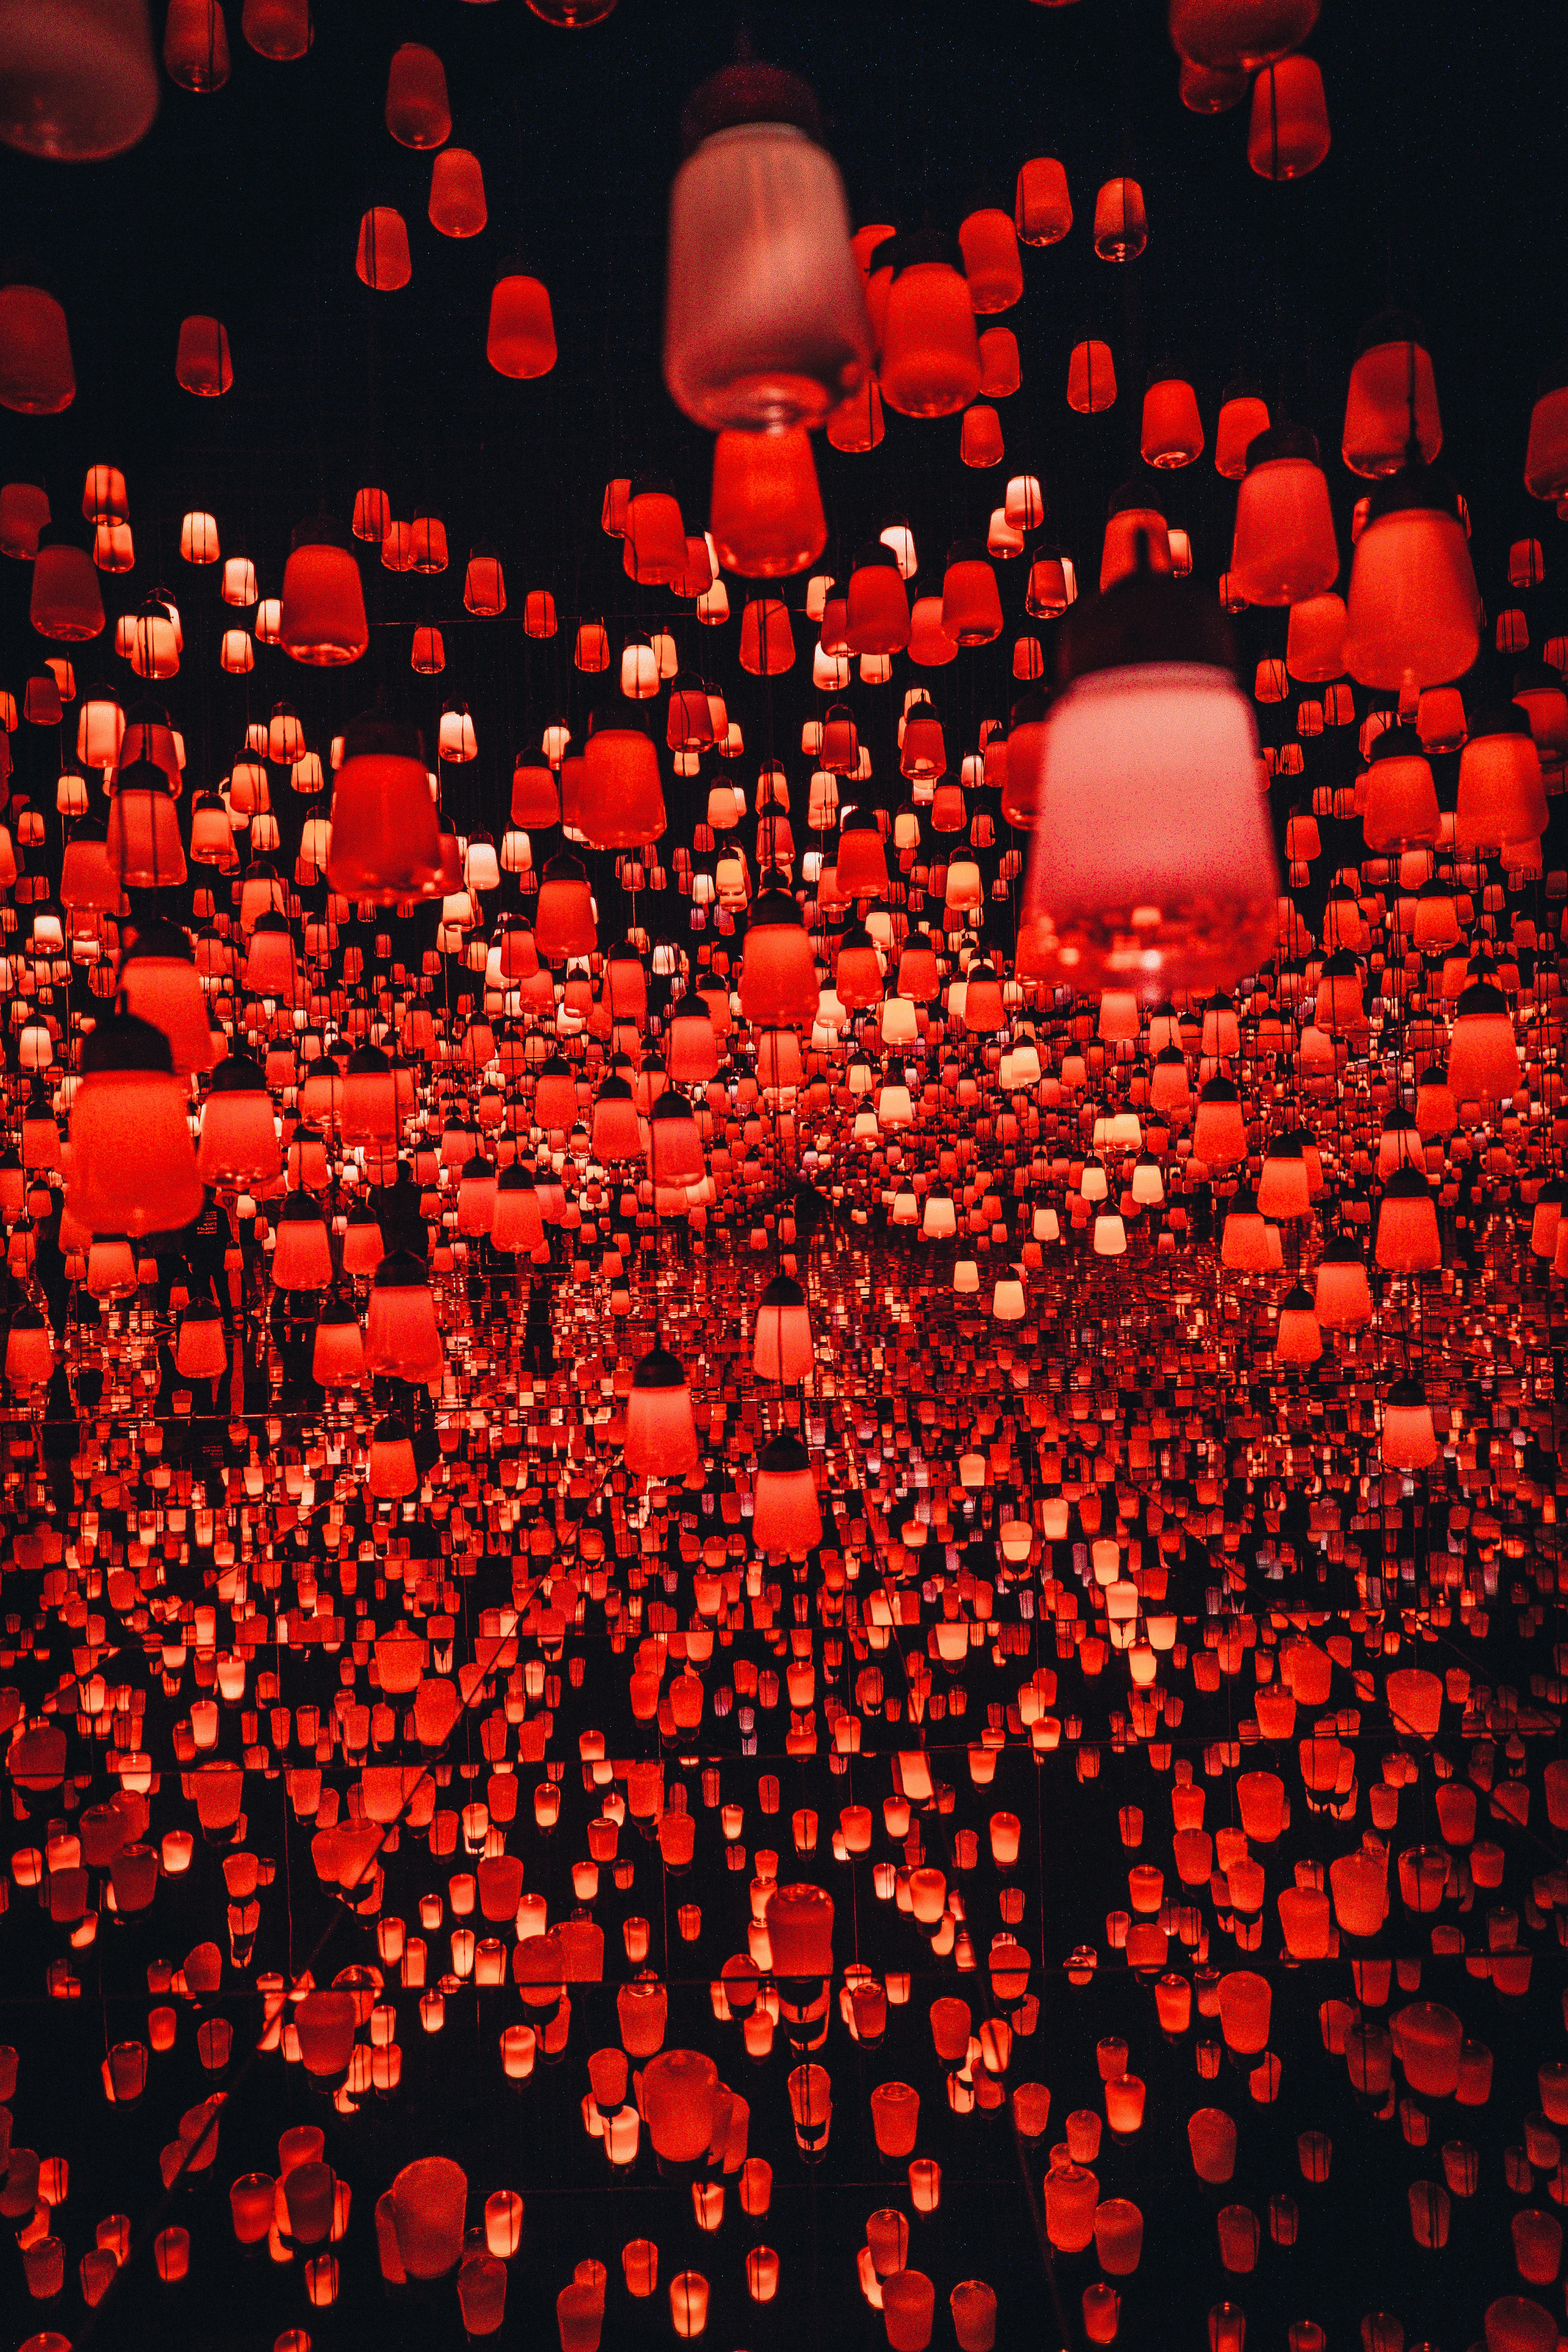
\includegraphics[width=6cm]{logo}}  %NEW: Changing logo
\def\extraspace{\vspace*{1.6cm}}
\makeatletter
\def\contactdetails{\faicon{phone} & \@telephone \\
                    \faicon{envelope} & \@email}
\makeatother

%%%% FRONT PAGE OF REPORTS

\def\reporttype{Report for}

\long\def\front#1#2#3{
\newpage
\begin{singlespacing}
\thispagestyle{empty}
\vspace*{-1.4cm}
\hspace*{-1.4cm}
\hbox to 16cm{
  \hbox to 6.5cm{\vbox to 14cm{\vbox to 25cm{
    \logo
    \vfill
    \parbox{6.3cm}{\raggedright
      \sf\color[rgb]{0.8, 0.7, 0.1 }    % NEW color 
      {\large\textbf{\name}}\par
      \vspace{.7cm}
      \tabcolsep=0.12cm\sf\small
      \begin{tabular}{@{}ll@{}}\contactdetails
      \end{tabular}
      \vspace*{0.3cm}\par
      ABN: \abn\par
    }
  }\vss}\hss}
  \hspace*{0.2cm}
  \hbox to 1cm{\vbox to 14cm{\rule{4pt}{26.8cm}\vss}\hss\hfill}  %NEW: Thicker line
  \hbox to 10cm{\vbox to 14cm{\vbox to 25cm{   
      \vspace*{3cm}\sf\raggedright
      \parbox{11cm}{\sf\raggedright\baselineskip=1.2cm
         \fontsize{24.88}{30}\color[rgb]{0, 0.29, 0.55}\sf\textbf{#1}}   % NEW: title color blue
      \par
      \vfill
      \large
      \vbox{\parskip=0.8cm #2}\par
      \vspace*{2cm}\par
      \reporttype\\[0.3cm]
      \hbox{#3}%\\[2cm]\
      \vspace*{1cm}
      {\large\sf\textbf{\Date~\Month~\Year}}
   }\vss}
  }}
\end{singlespacing}
\newpage
}

\makeatletter
\def\titlepage{\front{\expandafter{\@title}}{\@author}{\@organization}}
\makeatother

\usepackage{setspace}
\setstretch{1.5}

%% Any special functions or other packages can be loaded here.
\usepackage{booktabs}
\usepackage{longtable}
\usepackage{array}
\usepackage{multirow}
\usepackage{wrapfig}
\usepackage{float}
\usepackage{colortbl}
\usepackage{pdflscape}
\usepackage{tabu}
\usepackage{threeparttable}
\usepackage{threeparttablex}
\usepackage[normalem]{ulem}
\usepackage{makecell}
\usepackage{xcolor}


\begin{document}
\titlepage

\section*{Country Singapore and United States of America}

\begin{figure}
\centering
\includegraphics{report_files/figure-latex/sgp-usa-barchart-1.pdf}
\caption{\label{fig:sgp-usa-barchart}Total Deaths and Cases in SGP and USA from 01/03/2020 to 10/05/20}
\end{figure}

\begin{table}

\caption{\label{tab:summary-sgp-usa-week}Total Cases and Deaths, and Proportion of Deaths per week}
\centering
\begin{tabular}[t]{l|r|r|r|r|r}
\hline
country & week & month & cases\_per\_week & deaths\_per\_week & deaths\_prop\\
\hline
Singapore & 1 & 3 & 1.77 & 0.00 & 0.00\\
\hline
Singapore & 2 & 3 & 9.22 & 0.00 & 0.00\\
\hline
Singapore & 3 & 3 & 14.72 & 0.00 & 0.00\\
\hline
Singapore & 4 & 3 & 47.17 & 0.35 & 0.61\\
\hline
Singapore & 5 & 3 & 59.41 & 0.18 & 0.23\\
\hline
Singapore & 6 & 4 & 94.17 & 0.53 & 0.60\\
\hline
Singapore & 7 & 4 & 273.65 & 0.53 & 0.13\\
\hline
Singapore & 8 & 4 & 903.76 & 0.35 & 0.07\\
\hline
Singapore & 9 & 4 & 1136.61 & 0.53 & 0.06\\
\hline
Singapore & 10 & 4 & 216.01 & 0.00 & 0.00\\
\hline
Singapore & 10 & 5 & 556.34 & 0.71 & 0.13\\
\hline
Singapore & 11 & 5 & 652.99 & 0.35 & 0.05\\
\hline
United\_States\_of\_America & 1 & 3 & 0.11 & 0.02 & 22.30\\
\hline
United\_States\_of\_America & 2 & 3 & 1.99 & 0.06 & 4.53\\
\hline
United\_States\_of\_America & 3 & 3 & 11.94 & 0.18 & 1.46\\
\hline
United\_States\_of\_America & 4 & 3 & 127.71 & 1.54 & 1.21\\
\hline
United\_States\_of\_America & 5 & 3 & 361.22 & 7.89 & 2.15\\
\hline
United\_States\_of\_America & 6 & 4 & 622.24 & 23.90 & 3.85\\
\hline
United\_States\_of\_America & 7 & 4 & 655.32 & 38.70 & 5.92\\
\hline
United\_States\_of\_America & 8 & 4 & 627.07 & 57.74 & 9.18\\
\hline
United\_States\_of\_America & 9 & 4 & 613.44 & 41.89 & 7.19\\
\hline
United\_States\_of\_America & 10 & 4 & 157.28 & 14.43 & 9.15\\
\hline
United\_States\_of\_America & 10 & 5 & 430.13 & 24.35 & 5.62\\
\hline
United\_States\_of\_America & 11 & 5 & 394.01 & 30.14 & 7.71\\
\hline
\end{tabular}
\end{table}

\hypertarget{analysis}{%
\section{Analysis}\label{analysis}}

This report examines the confirmed COVID-19 cases and deaths recorded in Singapore and the United States (\emph{US}) from the start of March to 10 May 2020. Due to the significant difference in population size, the cases and deaths are scaled to per million people of each country's population for better comparison.

Figure \ref{fig:sgp-usa-barchart} displays the number of new cases in Singapore and \emph{US}. The x-axis shows the number of new cases and deaths on a given day and the y-axis represents each date. It is manifest that confirmed cases in both countries started to pick up in mid-March 2020. There was a gradual increase in new cases in \emph{US} in the last two weeks of March, where it stayed relatively constant to mid-May. In Singapore, an exponential increase in confirmed cases can be observed in mid-April', where the new confirmed cases overtook the US in relative terms (\emph{i.e.} per 1 million). Although the confirmed cases were higher in Singapore, the death rates in the \emph{US} were evidently greater, with Singapore staying relatively constant at 0\%.

To investigate further, we observe the start dates of the lockdown policy in each country. In Singapore, the lockdown started at the end of the first week of April, 07/04/2020 (\textcite{sgcb}). In USA, the effective dates were different in each state, California was the first to enforce it on 19/03/2020 while South Carolina was the last to carry it out on 07/04/2020 (\textcite{fowler2020effect}).

Based on Table \ref{tab:summary-sgp-usa-week}, Singapore's cases increased by a staggering 1103.91\% from the first week to the last week of April although lockdown and social distancing protocols were in effect. This surge is attributed to the surge in infections among migrant worker population staying in dormitories, which accounted for most of the confirmed cases (\textcite{sgcb2}).

On the other hand, \emph{US} cases nearly doubled (0.72\%) from approximately the end of March to the start of April. In contrary to Singapore's cases, confirmed cases in \emph{US} seemed to subside at the end of April 2020 after all states implemented lockdown policies. However, Table \ref{tab:summary-sgp-usa-week} demonstrated that the proportion of death rates in \emph{US} was not proportionate to the decrease in the cases per week.

\section*{Country Italy and USA}

\begin{figure}
\centering
\includegraphics{report_files/figure-latex/cases-plot-1.pdf}
\caption{\label{fig:cases-plot}2020 COVID-19 Cases in Italy and USA}
\end{figure}

Figure \ref{fig:cases-plot} reflects the number of COVID-19 cases in Italy and USA from January to May 2020. The total number of cases are reflected in the y axis, and the x axis represents the period (month). It is reflected in the figure that COVID-19 cases did not start in Italy and USA until March where there was no significant difference between the two countries. There was a slight increase in COVID-19 cases in April in Italy. However, the number of cases in the US rose significantly in April. By the end of April, the number of cases in the US is approximately four times larger in comparison to Italy. According to \autocite{vox} the number of COVID-19 cases in the US make up approximately a third of the world's cases.

\clearpage

\begin{table}

\caption{\label{tab:death-table}Top 5 Largest Number of Daily Deaths in Italy and USA}
\centering
\begin{tabular}[t]{l|l|r}
\hline
countriesAndTerritories & dateRep & deaths\\
\hline
United\_States\_of\_America & 16/04/2020 & 4928\\
\hline
United\_States\_of\_America & 18/04/2020 & 3770\\
\hline
United\_States\_of\_America & 24/04/2020 & 3179\\
\hline
United\_States\_of\_America & 30/04/2020 & 2611\\
\hline
United\_States\_of\_America & 22/04/2020 & 2524\\
\hline
\end{tabular}
\end{table}

Table \ref{tab:death-table} shows the top 5 largest daily in COVID-19 related deaths in Italy and USA. The table shows that the 5 largest amount of deaths occured in one day happened in the US. These mostly happened in the third and fourth week of April. The highest amount of daily deaths occured on the 16th of April, where 4,928 lose their lives.The second highest occured on the same week on the 18th of April with 3,770 number of deaths.

\section*{Country XX3 and YY3}

\clearpage

\hypertarget{citations}{%
\section{Citations}\label{citations}}

\begin{enumerate}
\def\labelenumi{\arabic{enumi}.}
\tightlist
\item
  \textcite{tidyverse}
\item
  \textcite{readr}
\item
  \textcite{KableExtra}
\item
  \textcite{bookdown}
\item
  \textcite{bookdown2}
\item
  \textcite{lubridate}
\end{enumerate}

\clearpage

\printbibliography

\end{document}

